\documentclass[]{book}
\usepackage{lmodern}
\usepackage{amssymb,amsmath}
\usepackage{ifxetex,ifluatex}
\usepackage{fixltx2e} % provides \textsubscript
\ifnum 0\ifxetex 1\fi\ifluatex 1\fi=0 % if pdftex
  \usepackage[T1]{fontenc}
  \usepackage[utf8]{inputenc}
\else % if luatex or xelatex
  \ifxetex
    \usepackage{mathspec}
  \else
    \usepackage{fontspec}
  \fi
  \defaultfontfeatures{Ligatures=TeX,Scale=MatchLowercase}
\fi
% use upquote if available, for straight quotes in verbatim environments
\IfFileExists{upquote.sty}{\usepackage{upquote}}{}
% use microtype if available
\IfFileExists{microtype.sty}{%
\usepackage{microtype}
\UseMicrotypeSet[protrusion]{basicmath} % disable protrusion for tt fonts
}{}
\usepackage[margin=1in]{geometry}
\usepackage{hyperref}
\hypersetup{unicode=true,
            pdftitle={bdDwC User Guide},
            pdfauthor={Authors: TBA},
            pdfborder={0 0 0},
            breaklinks=true}
\urlstyle{same}  % don't use monospace font for urls
\usepackage{natbib}
\bibliographystyle{apalike}
\usepackage{color}
\usepackage{fancyvrb}
\newcommand{\VerbBar}{|}
\newcommand{\VERB}{\Verb[commandchars=\\\{\}]}
\DefineVerbatimEnvironment{Highlighting}{Verbatim}{commandchars=\\\{\}}
% Add ',fontsize=\small' for more characters per line
\usepackage{framed}
\definecolor{shadecolor}{RGB}{248,248,248}
\newenvironment{Shaded}{\begin{snugshade}}{\end{snugshade}}
\newcommand{\KeywordTok}[1]{\textcolor[rgb]{0.13,0.29,0.53}{\textbf{#1}}}
\newcommand{\DataTypeTok}[1]{\textcolor[rgb]{0.13,0.29,0.53}{#1}}
\newcommand{\DecValTok}[1]{\textcolor[rgb]{0.00,0.00,0.81}{#1}}
\newcommand{\BaseNTok}[1]{\textcolor[rgb]{0.00,0.00,0.81}{#1}}
\newcommand{\FloatTok}[1]{\textcolor[rgb]{0.00,0.00,0.81}{#1}}
\newcommand{\ConstantTok}[1]{\textcolor[rgb]{0.00,0.00,0.00}{#1}}
\newcommand{\CharTok}[1]{\textcolor[rgb]{0.31,0.60,0.02}{#1}}
\newcommand{\SpecialCharTok}[1]{\textcolor[rgb]{0.00,0.00,0.00}{#1}}
\newcommand{\StringTok}[1]{\textcolor[rgb]{0.31,0.60,0.02}{#1}}
\newcommand{\VerbatimStringTok}[1]{\textcolor[rgb]{0.31,0.60,0.02}{#1}}
\newcommand{\SpecialStringTok}[1]{\textcolor[rgb]{0.31,0.60,0.02}{#1}}
\newcommand{\ImportTok}[1]{#1}
\newcommand{\CommentTok}[1]{\textcolor[rgb]{0.56,0.35,0.01}{\textit{#1}}}
\newcommand{\DocumentationTok}[1]{\textcolor[rgb]{0.56,0.35,0.01}{\textbf{\textit{#1}}}}
\newcommand{\AnnotationTok}[1]{\textcolor[rgb]{0.56,0.35,0.01}{\textbf{\textit{#1}}}}
\newcommand{\CommentVarTok}[1]{\textcolor[rgb]{0.56,0.35,0.01}{\textbf{\textit{#1}}}}
\newcommand{\OtherTok}[1]{\textcolor[rgb]{0.56,0.35,0.01}{#1}}
\newcommand{\FunctionTok}[1]{\textcolor[rgb]{0.00,0.00,0.00}{#1}}
\newcommand{\VariableTok}[1]{\textcolor[rgb]{0.00,0.00,0.00}{#1}}
\newcommand{\ControlFlowTok}[1]{\textcolor[rgb]{0.13,0.29,0.53}{\textbf{#1}}}
\newcommand{\OperatorTok}[1]{\textcolor[rgb]{0.81,0.36,0.00}{\textbf{#1}}}
\newcommand{\BuiltInTok}[1]{#1}
\newcommand{\ExtensionTok}[1]{#1}
\newcommand{\PreprocessorTok}[1]{\textcolor[rgb]{0.56,0.35,0.01}{\textit{#1}}}
\newcommand{\AttributeTok}[1]{\textcolor[rgb]{0.77,0.63,0.00}{#1}}
\newcommand{\RegionMarkerTok}[1]{#1}
\newcommand{\InformationTok}[1]{\textcolor[rgb]{0.56,0.35,0.01}{\textbf{\textit{#1}}}}
\newcommand{\WarningTok}[1]{\textcolor[rgb]{0.56,0.35,0.01}{\textbf{\textit{#1}}}}
\newcommand{\AlertTok}[1]{\textcolor[rgb]{0.94,0.16,0.16}{#1}}
\newcommand{\ErrorTok}[1]{\textcolor[rgb]{0.64,0.00,0.00}{\textbf{#1}}}
\newcommand{\NormalTok}[1]{#1}
\usepackage{longtable,booktabs}
\usepackage{graphicx,grffile}
\makeatletter
\def\maxwidth{\ifdim\Gin@nat@width>\linewidth\linewidth\else\Gin@nat@width\fi}
\def\maxheight{\ifdim\Gin@nat@height>\textheight\textheight\else\Gin@nat@height\fi}
\makeatother
% Scale images if necessary, so that they will not overflow the page
% margins by default, and it is still possible to overwrite the defaults
% using explicit options in \includegraphics[width, height, ...]{}
\setkeys{Gin}{width=\maxwidth,height=\maxheight,keepaspectratio}
\IfFileExists{parskip.sty}{%
\usepackage{parskip}
}{% else
\setlength{\parindent}{0pt}
\setlength{\parskip}{6pt plus 2pt minus 1pt}
}
\setlength{\emergencystretch}{3em}  % prevent overfull lines
\providecommand{\tightlist}{%
  \setlength{\itemsep}{0pt}\setlength{\parskip}{0pt}}
\setcounter{secnumdepth}{5}
% Redefines (sub)paragraphs to behave more like sections
\ifx\paragraph\undefined\else
\let\oldparagraph\paragraph
\renewcommand{\paragraph}[1]{\oldparagraph{#1}\mbox{}}
\fi
\ifx\subparagraph\undefined\else
\let\oldsubparagraph\subparagraph
\renewcommand{\subparagraph}[1]{\oldsubparagraph{#1}\mbox{}}
\fi

%%% Use protect on footnotes to avoid problems with footnotes in titles
\let\rmarkdownfootnote\footnote%
\def\footnote{\protect\rmarkdownfootnote}

%%% Change title format to be more compact
\usepackage{titling}

% Create subtitle command for use in maketitle
\newcommand{\subtitle}[1]{
  \posttitle{
    \begin{center}\large#1\end{center}
    }
}

\setlength{\droptitle}{-2em}

  \title{\texttt{bdDwC} User Guide}
    \pretitle{\vspace{\droptitle}\centering\huge}
  \posttitle{\par}
    \author{Authors: TBA}
    \preauthor{\centering\large\emph}
  \postauthor{\par}
      \predate{\centering\large\emph}
  \postdate{\par}
    \date{2018-09-03}

\usepackage{booktabs}

\usepackage{amsthm}
\newtheorem{theorem}{Theorem}[chapter]
\newtheorem{lemma}{Lemma}[chapter]
\theoremstyle{definition}
\newtheorem{definition}{Definition}[chapter]
\newtheorem{corollary}{Corollary}[chapter]
\newtheorem{proposition}{Proposition}[chapter]
\theoremstyle{definition}
\newtheorem{example}{Example}[chapter]
\theoremstyle{definition}
\newtheorem{exercise}{Exercise}[chapter]
\theoremstyle{remark}
\newtheorem*{remark}{Remark}
\newtheorem*{solution}{Solution}
\begin{document}
\maketitle

{
\setcounter{tocdepth}{1}
\tableofcontents
}
\chapter*{Introduction}\label{introduction}
\addcontentsline{toc}{chapter}{Introduction}

\textbf{{{[} TBA {]}}}

\subsubsection*{Motivation}\label{motivation}
\addcontentsline{toc}{subsubsection}{Motivation}

\textbf{{{[} TBA {]}}}

\chapter{\texorpdfstring{Installing
\texttt{bdDwC}}{Installing bdDwC}}\label{installing-bddwc}

\begin{center}\rule{0.5\linewidth}{\linethickness}\end{center}

\section{Stable version from CRAN}\label{stable-version-from-cran}

\textbf{{{[} Need To Be Updated! {]}}}

\begin{Shaded}
\begin{Highlighting}[]
\CommentTok{# The easiest way to get bdDwC is to install the whole bdverse:}
\KeywordTok{install.packages}\NormalTok{(}\StringTok{"bdverse"}\NormalTok{)}
\end{Highlighting}
\end{Shaded}

\begin{Shaded}
\begin{Highlighting}[]
\CommentTok{# Alternatively, install just bdDwC:}
\KeywordTok{install.packages}\NormalTok{(}\StringTok{"bdDwC"}\NormalTok{)}
\end{Highlighting}
\end{Shaded}

\section{Development version from
GitHub}\label{development-version-from-github}

Windows users install
\href{https://cran.r-project.org/bin/windows/Rtools/}{Rtools} first.

\begin{Shaded}
\begin{Highlighting}[]
\KeywordTok{install.packages}\NormalTok{(}\StringTok{"devtools"}\NormalTok{)}
\NormalTok{devtools}\OperatorTok{::}\KeywordTok{install_github}\NormalTok{(}\StringTok{"bd-R/bdDwC"}\NormalTok{)}
\end{Highlighting}
\end{Shaded}

\section{Possible problems \&
solutions}\label{possible-problems-solutions}

\textbf{{{[} TBA {]}}}

\subsection{???}\label{section}

TBA

\subsection{????}\label{section-1}

TBA

\chapter{The shiny app}\label{the-shiny-app}

\begin{center}\rule{0.5\linewidth}{\linethickness}\end{center}

\section{Launching the app}\label{launching-the-app}

\begin{Shaded}
\begin{Highlighting}[]
\KeywordTok{library}\NormalTok{(bdDwC) }\CommentTok{# Uplaod package library}
\KeywordTok{runDwC}\NormalTok{() }\CommentTok{# Launch the app}
\end{Highlighting}
\end{Shaded}

\section{App overview}\label{app-overview}

\textbf{{{[} Need To Be Updated! {]}}}

\begin{figure}
\centering
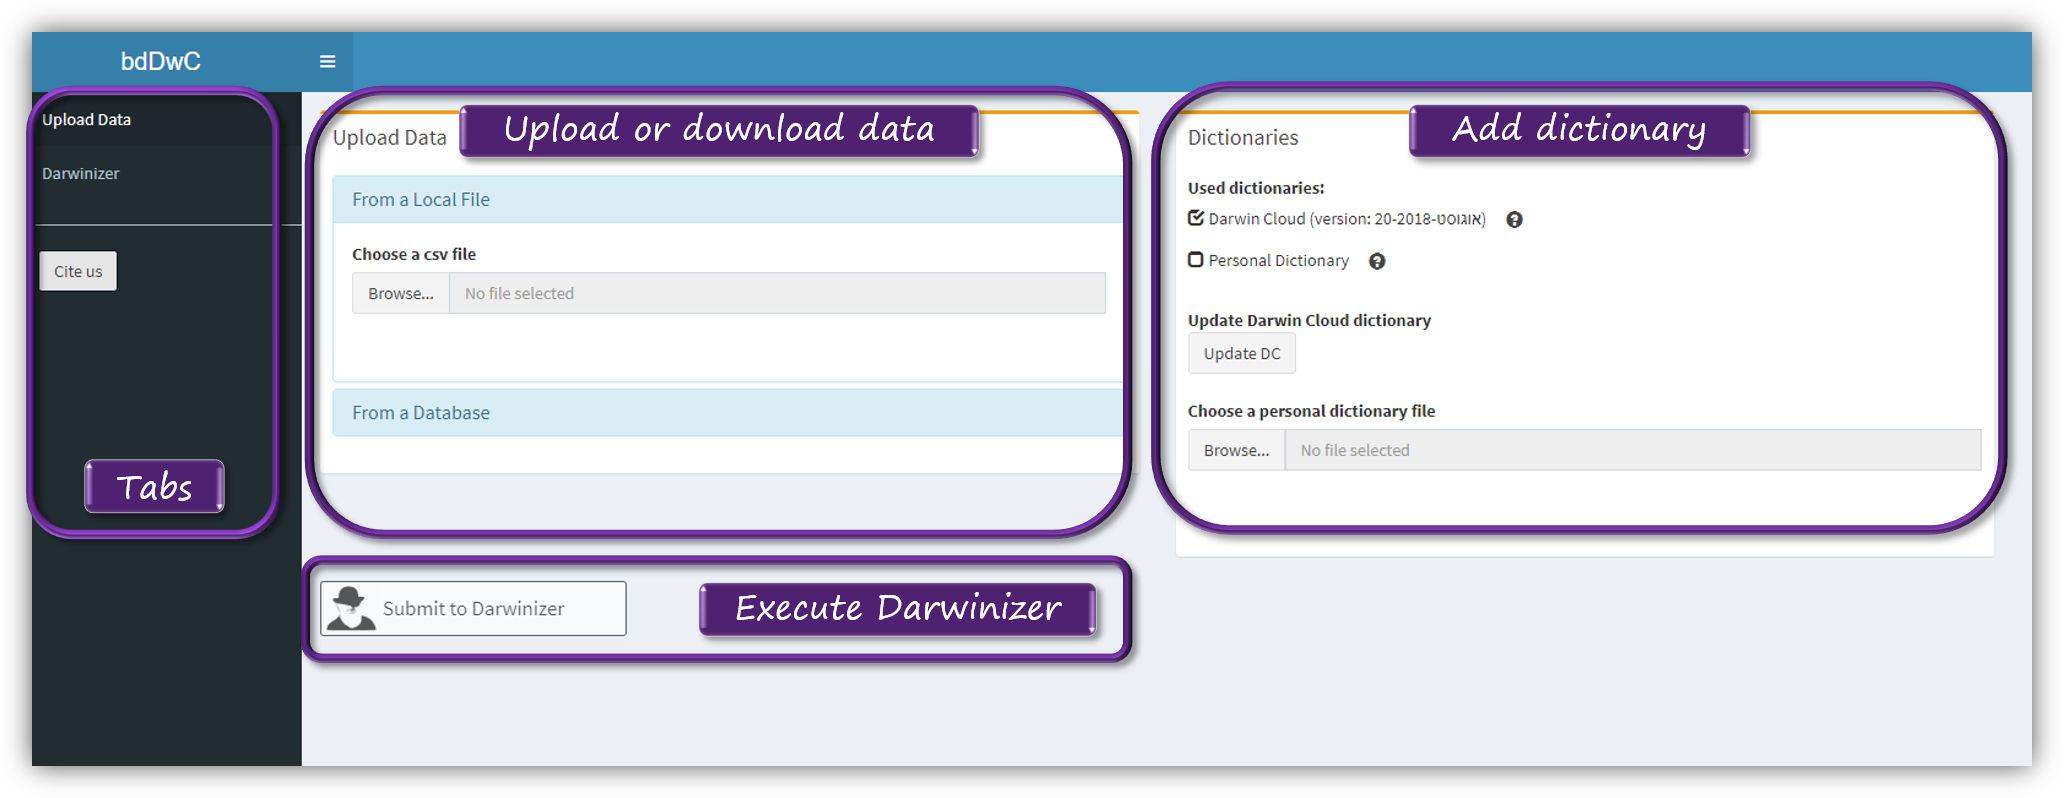
\includegraphics{img/bdDwC_Getting_started.png}
\caption{bdDwC App Overview}
\end{figure}

In the first screen, you'll need to upload or download your biodiversity
data; choose dictionary and run the Darwinizer.

\section{Data upload}\label{data-upload}

\subsection{From a local file}\label{from-a-local-file}

A CSV file or a Darwin Core Archive (DwC-A) zip file can be uploaded.

\textbf{Local file size cannot exceed {1GB {[}?{]}}}

\textbf{{{[} Need To Be Updated! {]}}}

\begin{figure}
\centering
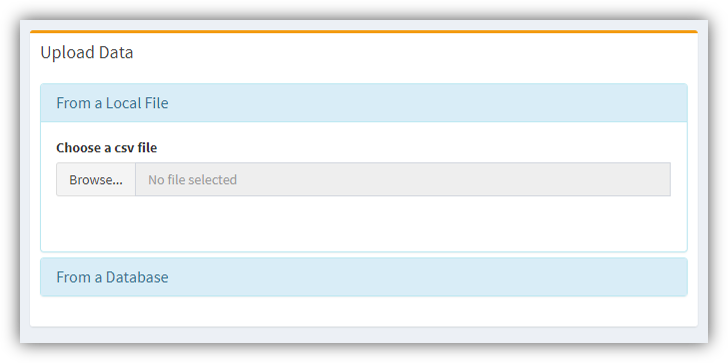
\includegraphics{img/bdDwC_Up-local_file.png}
\caption{Data upload from a local file}
\end{figure}

\subsection{From an online database}\label{from-an-online-database}

Also, data can be retrieved directly from various online biodiversity
databases. You need only to:

\begin{itemize}
\tightlist
\item
  Select the database
\item
  Specify the desired scientific name.
\item
  Specify the number of records (upper limit of 50,000).
\item
  Check the box if records must have coordinates.
\item
  Wait for data to be downloaded.
\end{itemize}

\textbf{{{[} Need To Be Updated! {]}}}

\begin{figure}
\centering
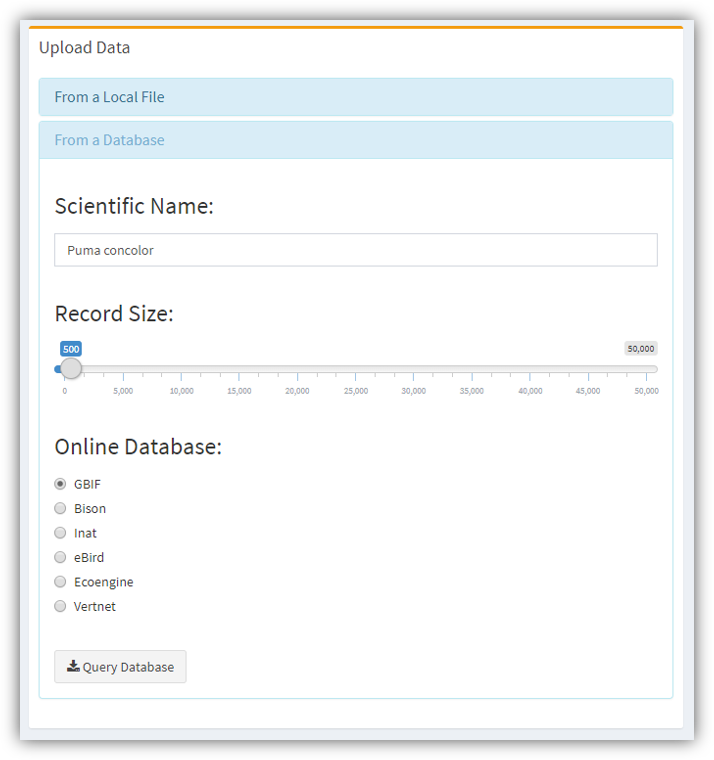
\includegraphics{img/bdDwC_Up-database.png}
\caption{Data upload from online biodiversity databases}
\end{figure}

\section{Dictionaries}\label{dictionaries}

A dictionary is a key component when Darwinizing a dataset. It's
basically a lookup table that lists a possible variation of field name
and it corresponding DwC name.

\hypertarget{the-darwin-cloud-dictionary}{\subsection{The Darwin Cloud
dictionary}\label{the-darwin-cloud-dictionary}}

The Darwin Cloud dictionary \citep{DarwinCloud}, is a lookup table that
accumulates different variations in DwC field names from different
publishers. This valuable dictionary was created and is maintained by
the Kurator project (\url{http://kurator.acis.ufl.edu/kurator-web/}),
which provides workflow tools for data quality improvement of
biodiversity data, via a user-friendly web interface.

\subsubsection*{Updating the Darwin
Cloud}\label{updating-the-darwin-cloud}
\addcontentsline{toc}{subsubsection}{Updating the Darwin Cloud}

It's recommended to update the Darwin Cloud file. This can be done
easily by clicking the \textbf{Update DC} button.

\textbf{{{[} Need To Be Updated! {]}}}

\begin{figure}
\centering
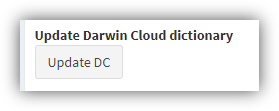
\includegraphics{img/bdDwC_update-DC.png}
\caption{Updating the Darwin Cloud}
\end{figure}

\subsection{Your own dictionary}\label{your-own-dictionary}

It's also possible to add your own dictionary by simply creating a CSV
file with two columns, one for the Field Names and one for the Standard
Names.

\textbf{{{[} Need To Be Updated! {]}}}

\begin{figure}
\centering
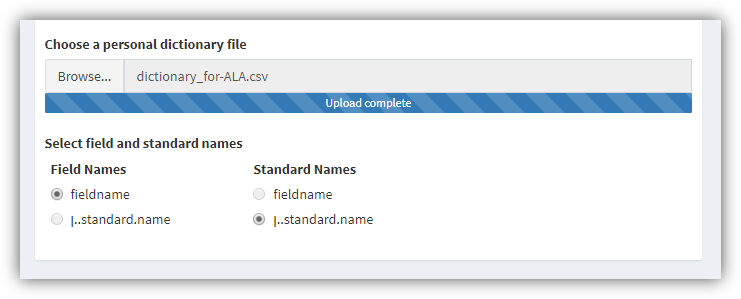
\includegraphics{img/bdDwC_personal_dictionary.png}
\caption{Uploading your own dictionary}
\end{figure}

\section{Darwinizing your dataset}\label{darwinizing-your-dataset}

Once a dataset is uploaded, the `Submit to Darwinizer' button is
activated, Clicking it will Darwinize the dataset.

\textbf{{{[} Need To Be Updated! {]}}}

\begin{figure}
\centering
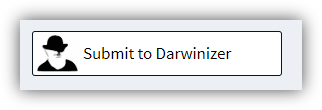
\includegraphics{img/bdDwC_Submit.png}
\caption{Submit to Darwinizer button}
\end{figure}

\section{Darwinizer results}\label{darwinizer-results}

\subsection{Results page overwiew}\label{results-page-overwiew}

\textbf{{{[} Need To Be Updated! {]}}}

\begin{figure}
\centering
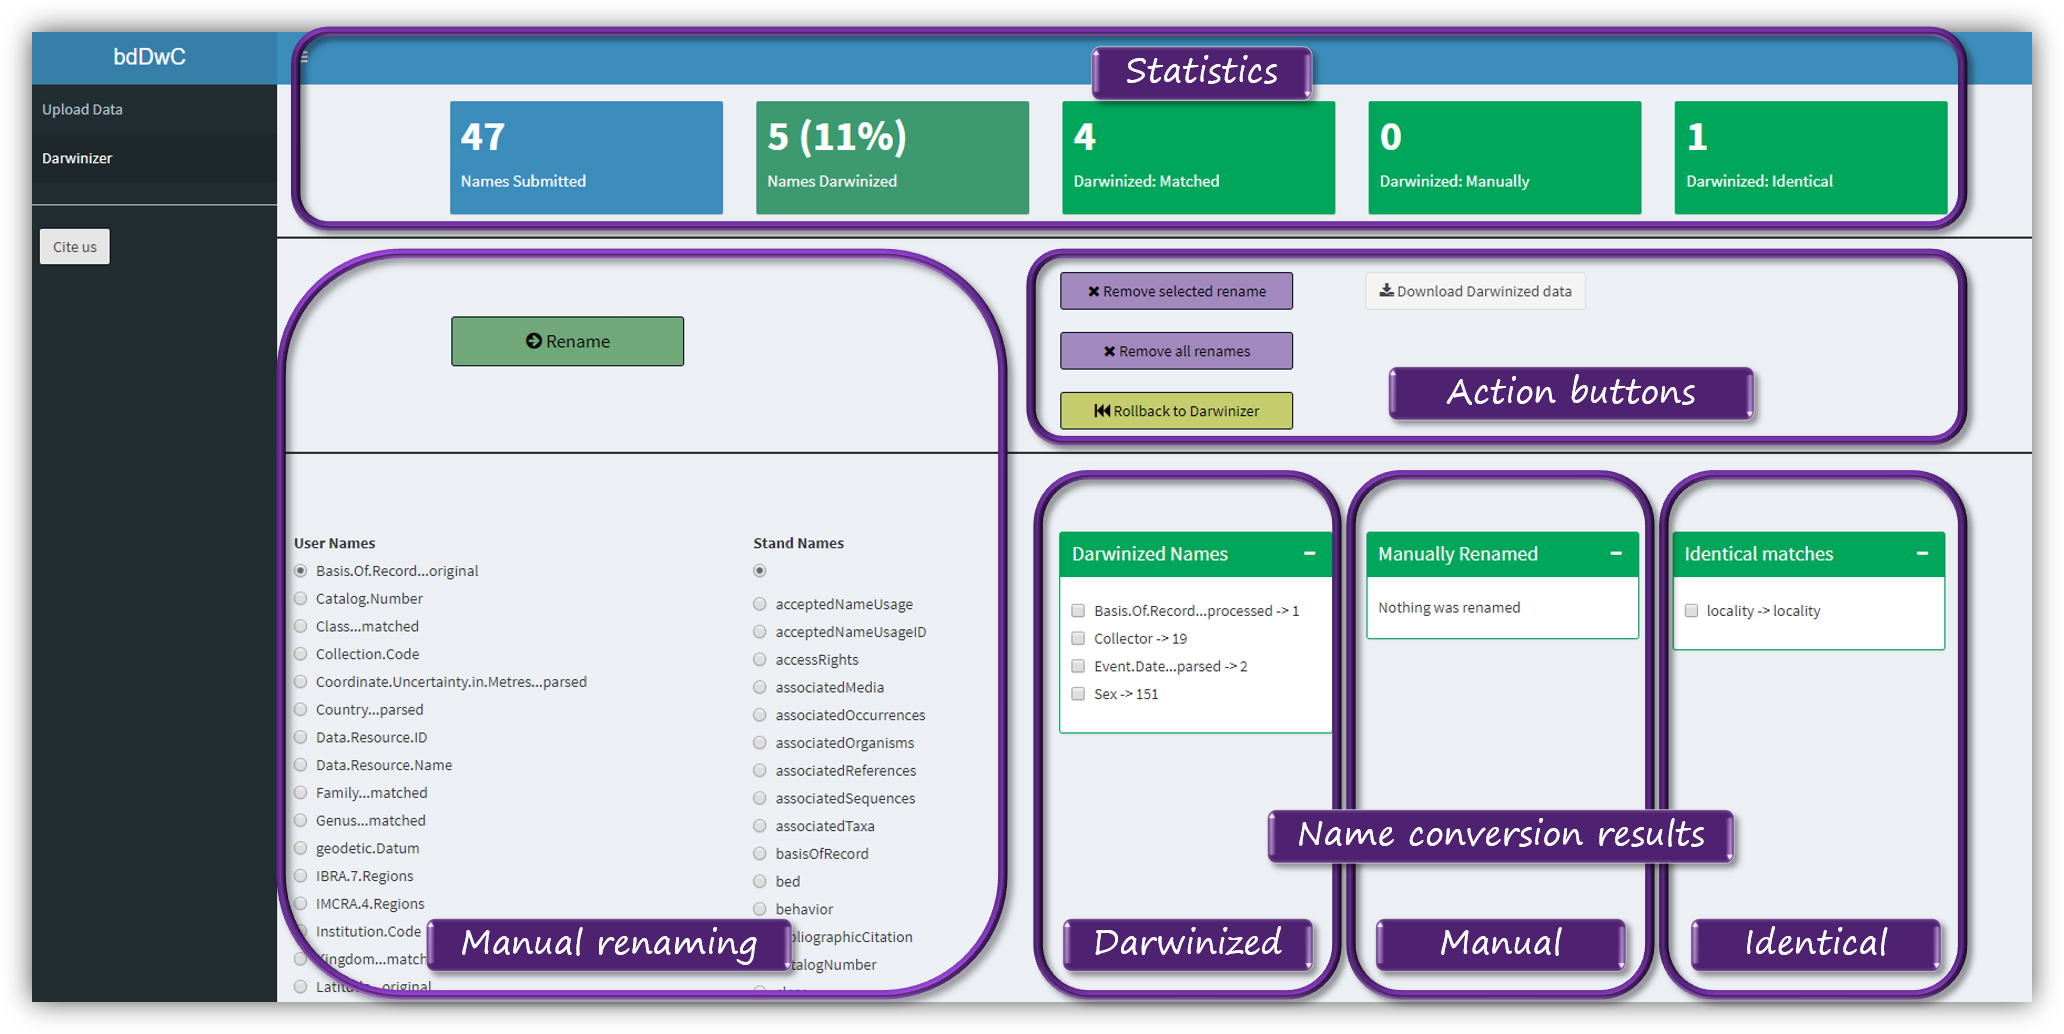
\includegraphics{img/bdDwC_Darwinizer_results.png}
\caption{Darwinizer results}
\end{figure}

Manually renaming field names can be done very easily, just choose the
two corresponding fields and click the Rename button.

\textbf{{{[} Need To Be Updated! {]}}}

\begin{figure}
\centering
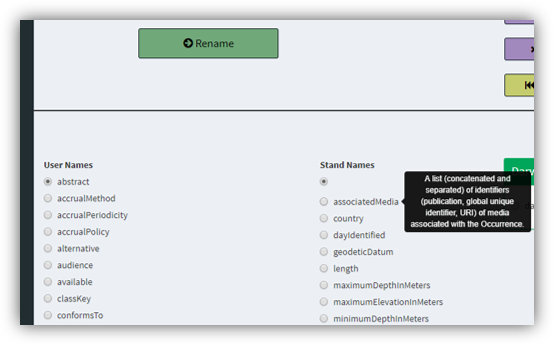
\includegraphics{img/bdDwC_Manual_rename.png}
\caption{Manually renaming fields}
\end{figure}

Hovering over a DwC standard name will display its description.

\section{Download your Darwinized
data}\label{download-your-darwinized-data}

\textbf{{{[} Need To Be Updated! {]}}}

\section{Closing the app}\label{closing-the-app}

\section{References}\label{references}

\chapter{Command line operations}\label{command-line-operations}

\begin{center}\rule{0.5\linewidth}{\linethickness}\end{center}

\section{Load package}\label{load-package}

Load the \texttt{bdDwC} package

\begin{Shaded}
\begin{Highlighting}[]
    \KeywordTok{library}\NormalTok{(bdDwC)}
\end{Highlighting}
\end{Shaded}

\section{Darwinizing a dataset}\label{darwinizing-a-dataset}

\texttt{bdDwC} contains Indian Reptile dataset
\texttt{bdDwC:::dataReptiles}.

The function to Darwinize a dataset is\texttt{darwinizeNames} (replace
\texttt{bdDwC:::dataReptiles} with wanted dataset):

\begin{Shaded}
\begin{Highlighting}[]
\NormalTok{result <-}\StringTok{ }\KeywordTok{darwinizeNames}\NormalTok{(}\DataTypeTok{dataUser =}\NormalTok{ bdDwC}\OperatorTok{:::}\NormalTok{dataReptiles,}
                            \DataTypeTok{dataDWC   =}\NormalTok{ bdDwC}\OperatorTok{:::}\NormalTok{dataDarwinCloud}\OperatorTok{$}\NormalTok{data)}
\end{Highlighting}
\end{Shaded}

You can replace \texttt{bdDwC:::dataReptiles} with your dataset

Rename your dataset field names to Darwinized names using
\texttt{renameUserData}:

\begin{Shaded}
\begin{Highlighting}[]
\KeywordTok{renameUserData}\NormalTok{(bdDwC}\OperatorTok{:::}\NormalTok{dataReptiles, result)}
\end{Highlighting}
\end{Shaded}

\section{\texorpdfstring{Updating
\protect\hyperlink{the-darwin-cloud-dictionary}{the Darwin Cloud
dictionary}}{Updating the Darwin Cloud dictionary}}\label{updating-the-darwin-cloud-dictionary}

To get newest version of Darwin Cloud Data run:

\begin{Shaded}
\begin{Highlighting}[]
\KeywordTok{downloadCloudData}\NormalTok{()}
\end{Highlighting}
\end{Shaded}

which will download data from the remote repository and extract field
and standard names.

\chapter{Examples}\label{examples}

\begin{center}\rule{0.5\linewidth}{\linethickness}\end{center}

\textbf{{{[} TBA {]}}}

I'm thinking to show the Darwinizer app with four distinct datasets:

\begin{enumerate}
\def\labelenumi{\arabic{enumi}.}
\tightlist
\item
  ALA dataset in DwC format
\item
  ALA dataset in legacy format
\item
  VertNet dataset
\item
  GBIF dataset
\end{enumerate}

\chapter{References}\label{references-1}

\chapter{Getting your feedback}\label{getting-your-feedback}

\begin{center}\rule{0.5\linewidth}{\linethickness}\end{center}

Loading\ldots{}

\section{Report a bug}\label{report-a-bug}

Submit an issue at \url{https://github.com/bd-R/bdDwC/issues}

\section{Contribute}\label{contribute}

Contribute: \url{https://github.com/bd-R/bdDwC}

Join: \url{https://bd-r-group.slack.com}

\chapter{\texorpdfstring{\texttt{bdDwC}
citation}{bdDwC citation}}\label{bddwc-citation}

\begin{center}\rule{0.5\linewidth}{\linethickness}\end{center}

\begin{Shaded}
\begin{Highlighting}[]
\KeywordTok{citation}\NormalTok{(}\StringTok{"bdDwC"}\NormalTok{)}
\end{Highlighting}
\end{Shaded}

\begin{verbatim}
## 
## To cite package 'bdDwC' in publications use:
## 
##   Povilas Gibas, Tomer Gueta, Vijay Barve, Thiloshon Nagarajah and
##   Yohay Carmel (2018). bdDwC: Darwinizer: Darwin Core (DwC) Field
##   Names Standardization. R package version 0.1.15.
## 
## A BibTeX entry for LaTeX users is
## 
##   @Manual{,
##     title = {bdDwC: Darwinizer: Darwin Core (DwC) Field Names Standardization},
##     author = {Povilas Gibas and Tomer Gueta and Vijay Barve and Thiloshon Nagarajah and Yohay Carmel},
##     year = {2018},
##     note = {R package version 0.1.15},
##   }
\end{verbatim}

\chapter{Learn more about Darwin
Core}\label{learn-more-about-darwin-core}

\begin{center}\rule{0.5\linewidth}{\linethickness}\end{center}

\begin{itemize}
\tightlist
\item
  \href{https://github.com/tdwg/dwc-qa/wiki/Webinars\%20target=\%22_blank\%22}{Darwin
  Core Hour webinar series}
\item
  \href{https://github.com/tdwg/dwc-qa/wiki\%20target=\%22_blank\%22}{The
  Darwin Core Questions \& Answers wiki}
\item
  \href{https://www.gbif.org/darwin-core\%20target=\%22_blank\%22}{GBIF:
  What is Darwin Core, and why does it matter?}
\item
  Darwin Core: An Evolving Community-Developed Biodiversity Data
  Standard \citep{DwC-paper}
\end{itemize}

\section{References}\label{references-2}

\bibliography{bib/book.bib,bib/DarwinCloud.bib,bib/DwC-paper.bib}


\end{document}
